% Options for packages loaded elsewhere
% Options for packages loaded elsewhere
\PassOptionsToPackage{unicode}{hyperref}
\PassOptionsToPackage{hyphens}{url}
%
\documentclass[
  chinese,
  11pt,
  a4paper,
]{book}
\usepackage{xcolor}
\usepackage{amsmath,amssymb}
\setcounter{secnumdepth}{5}
\usepackage{iftex}
\ifPDFTeX
  \usepackage[T1]{fontenc}
  \usepackage[utf8]{inputenc}
  \usepackage{textcomp} % provide euro and other symbols
\else % if luatex or xetex
  \usepackage{unicode-math} % this also loads fontspec
  \defaultfontfeatures{Scale=MatchLowercase}
  \defaultfontfeatures[\rmfamily]{Ligatures=TeX,Scale=1}
\fi
\usepackage{lmodern}
\ifPDFTeX\else
  % xetex/luatex font selection
  \setmainfont[]{Noto Serif TC}
  \setmonofont[Scale=0.8]{Fira Code}
\fi
% Use upquote if available, for straight quotes in verbatim environments
\IfFileExists{upquote.sty}{\usepackage{upquote}}{}
\IfFileExists{microtype.sty}{% use microtype if available
  \usepackage[]{microtype}
  \UseMicrotypeSet[protrusion]{basicmath} % disable protrusion for tt fonts
}{}
\usepackage{setspace}
\makeatletter
\@ifundefined{KOMAClassName}{% if non-KOMA class
  \IfFileExists{parskip.sty}{%
    \usepackage{parskip}
  }{% else
    \setlength{\parindent}{0pt}
    \setlength{\parskip}{6pt plus 2pt minus 1pt}}
}{% if KOMA class
  \KOMAoptions{parskip=half}}
\makeatother
% Make \paragraph and \subparagraph free-standing
\makeatletter
\ifx\paragraph\undefined\else
  \let\oldparagraph\paragraph
  \renewcommand{\paragraph}{
    \@ifstar
      \xxxParagraphStar
      \xxxParagraphNoStar
  }
  \newcommand{\xxxParagraphStar}[1]{\oldparagraph*{#1}\mbox{}}
  \newcommand{\xxxParagraphNoStar}[1]{\oldparagraph{#1}\mbox{}}
\fi
\ifx\subparagraph\undefined\else
  \let\oldsubparagraph\subparagraph
  \renewcommand{\subparagraph}{
    \@ifstar
      \xxxSubParagraphStar
      \xxxSubParagraphNoStar
  }
  \newcommand{\xxxSubParagraphStar}[1]{\oldsubparagraph*{#1}\mbox{}}
  \newcommand{\xxxSubParagraphNoStar}[1]{\oldsubparagraph{#1}\mbox{}}
\fi
\makeatother

\usepackage{color}
\usepackage{fancyvrb}
\newcommand{\VerbBar}{|}
\newcommand{\VERB}{\Verb[commandchars=\\\{\}]}
\DefineVerbatimEnvironment{Highlighting}{Verbatim}{commandchars=\\\{\}}
% Add ',fontsize=\small' for more characters per line
\usepackage{framed}
\definecolor{shadecolor}{RGB}{241,243,245}
\newenvironment{Shaded}{\begin{snugshade}}{\end{snugshade}}
\newcommand{\AlertTok}[1]{\textcolor[rgb]{0.68,0.00,0.00}{#1}}
\newcommand{\AnnotationTok}[1]{\textcolor[rgb]{0.37,0.37,0.37}{#1}}
\newcommand{\AttributeTok}[1]{\textcolor[rgb]{0.40,0.45,0.13}{#1}}
\newcommand{\BaseNTok}[1]{\textcolor[rgb]{0.68,0.00,0.00}{#1}}
\newcommand{\BuiltInTok}[1]{\textcolor[rgb]{0.00,0.23,0.31}{#1}}
\newcommand{\CharTok}[1]{\textcolor[rgb]{0.13,0.47,0.30}{#1}}
\newcommand{\CommentTok}[1]{\textcolor[rgb]{0.37,0.37,0.37}{#1}}
\newcommand{\CommentVarTok}[1]{\textcolor[rgb]{0.37,0.37,0.37}{\textit{#1}}}
\newcommand{\ConstantTok}[1]{\textcolor[rgb]{0.56,0.35,0.01}{#1}}
\newcommand{\ControlFlowTok}[1]{\textcolor[rgb]{0.00,0.23,0.31}{\textbf{#1}}}
\newcommand{\DataTypeTok}[1]{\textcolor[rgb]{0.68,0.00,0.00}{#1}}
\newcommand{\DecValTok}[1]{\textcolor[rgb]{0.68,0.00,0.00}{#1}}
\newcommand{\DocumentationTok}[1]{\textcolor[rgb]{0.37,0.37,0.37}{\textit{#1}}}
\newcommand{\ErrorTok}[1]{\textcolor[rgb]{0.68,0.00,0.00}{#1}}
\newcommand{\ExtensionTok}[1]{\textcolor[rgb]{0.00,0.23,0.31}{#1}}
\newcommand{\FloatTok}[1]{\textcolor[rgb]{0.68,0.00,0.00}{#1}}
\newcommand{\FunctionTok}[1]{\textcolor[rgb]{0.28,0.35,0.67}{#1}}
\newcommand{\ImportTok}[1]{\textcolor[rgb]{0.00,0.46,0.62}{#1}}
\newcommand{\InformationTok}[1]{\textcolor[rgb]{0.37,0.37,0.37}{#1}}
\newcommand{\KeywordTok}[1]{\textcolor[rgb]{0.00,0.23,0.31}{\textbf{#1}}}
\newcommand{\NormalTok}[1]{\textcolor[rgb]{0.00,0.23,0.31}{#1}}
\newcommand{\OperatorTok}[1]{\textcolor[rgb]{0.37,0.37,0.37}{#1}}
\newcommand{\OtherTok}[1]{\textcolor[rgb]{0.00,0.23,0.31}{#1}}
\newcommand{\PreprocessorTok}[1]{\textcolor[rgb]{0.68,0.00,0.00}{#1}}
\newcommand{\RegionMarkerTok}[1]{\textcolor[rgb]{0.00,0.23,0.31}{#1}}
\newcommand{\SpecialCharTok}[1]{\textcolor[rgb]{0.37,0.37,0.37}{#1}}
\newcommand{\SpecialStringTok}[1]{\textcolor[rgb]{0.13,0.47,0.30}{#1}}
\newcommand{\StringTok}[1]{\textcolor[rgb]{0.13,0.47,0.30}{#1}}
\newcommand{\VariableTok}[1]{\textcolor[rgb]{0.07,0.07,0.07}{#1}}
\newcommand{\VerbatimStringTok}[1]{\textcolor[rgb]{0.13,0.47,0.30}{#1}}
\newcommand{\WarningTok}[1]{\textcolor[rgb]{0.37,0.37,0.37}{\textit{#1}}}

\usepackage{longtable,booktabs,array}
\usepackage{calc} % for calculating minipage widths
% Correct order of tables after \paragraph or \subparagraph
\usepackage{etoolbox}
\makeatletter
\patchcmd\longtable{\par}{\if@noskipsec\mbox{}\fi\par}{}{}
\makeatother
% Allow footnotes in longtable head/foot
\IfFileExists{footnotehyper.sty}{\usepackage{footnotehyper}}{\usepackage{footnote}}
\makesavenoteenv{longtable}
\usepackage{graphicx}
\makeatletter
\newsavebox\pandoc@box
\newcommand*\pandocbounded[1]{% scales image to fit in text height/width
  \sbox\pandoc@box{#1}%
  \Gscale@div\@tempa{\textheight}{\dimexpr\ht\pandoc@box+\dp\pandoc@box\relax}%
  \Gscale@div\@tempb{\linewidth}{\wd\pandoc@box}%
  \ifdim\@tempb\p@<\@tempa\p@\let\@tempa\@tempb\fi% select the smaller of both
  \ifdim\@tempa\p@<\p@\scalebox{\@tempa}{\usebox\pandoc@box}%
  \else\usebox{\pandoc@box}%
  \fi%
}
% Set default figure placement to htbp
\def\fps@figure{htbp}
\makeatother



\ifLuaTeX
\usepackage[bidi=basic,provide=*]{babel}
\else
\usepackage[bidi=default,provide=*]{babel}
\fi
\ifPDFTeX
\else
\babelfont{rm}[]{Noto Serif TC}
\fi
% get rid of language-specific shorthands (see #6817):
\let\LanguageShortHands\languageshorthands
\def\languageshorthands#1{}


\setlength{\emergencystretch}{3em} % prevent overfull lines

\providecommand{\tightlist}{%
  \setlength{\itemsep}{0pt}\setlength{\parskip}{0pt}}



 


\usepackage{lipsum}
\usepackage{setspace}
%\onehalfspacing
%\setlength{\parskip}{1.5em}   % 段落之間距離
%\setlength{\intextsep}{1.5em}   % 圖片與文字間距
%\setlength{\textfloatsep}{1.5em} % 浮動圖與上下文字間距
%\setlength{\abovecaptionskip}{0.5em} % caption 與表格/圖片間距
%\setlength{\belowcaptionskip}{0.8em}

\fvset{baselinestretch=1, xleftmargin=2em, framesep=8mm, vspace=2em}

\usepackage{etoolbox}
\BeforeBeginEnvironment{Shaded}{\vspace{1em}}
\AfterEndEnvironment{Shaded}{\vspace{0.25em}}

\usepackage{enumitem}
\setlist{itemsep=1pt, topsep=0.6em}  % 每個項目與清單上下間距
\makeatletter
\@ifpackageloaded{bookmark}{}{\usepackage{bookmark}}
\makeatother
\makeatletter
\@ifpackageloaded{caption}{}{\usepackage{caption}}
\AtBeginDocument{%
\ifdefined\contentsname
  \renewcommand*\contentsname{目錄}
\else
  \newcommand\contentsname{目錄}
\fi
\ifdefined\listfigurename
  \renewcommand*\listfigurename{圖目錄}
\else
  \newcommand\listfigurename{圖目錄}
\fi
\ifdefined\listtablename
  \renewcommand*\listtablename{表目錄}
\else
  \newcommand\listtablename{表目錄}
\fi
\ifdefined\figurename
  \renewcommand*\figurename{圖}
\else
  \newcommand\figurename{圖}
\fi
\ifdefined\tablename
  \renewcommand*\tablename{表}
\else
  \newcommand\tablename{表}
\fi
}
\@ifpackageloaded{float}{}{\usepackage{float}}
\floatstyle{ruled}
\@ifundefined{c@chapter}{\newfloat{codelisting}{h}{lop}}{\newfloat{codelisting}{h}{lop}[chapter]}
\floatname{codelisting}{列表}
\newcommand*\listoflistings{\listof{codelisting}{列表目錄}}
\makeatother
\makeatletter
\makeatother
\makeatletter
\@ifpackageloaded{caption}{}{\usepackage{caption}}
\@ifpackageloaded{subcaption}{}{\usepackage{subcaption}}
\makeatother
\makeatletter
\@ifpackageloaded{tikz}{}{\usepackage{tikz}}
\makeatother
        \newcommand*\circled[1]{\tikz[baseline=(char.base)]{
          \node[shape=circle,draw,inner sep=1pt] (char) {{\scriptsize#1}};}}  
                  
\usepackage{bookmark}
\IfFileExists{xurl.sty}{\usepackage{xurl}}{} % add URL line breaks if available
\urlstyle{same}
\hypersetup{
  pdftitle={我的 Quarto 書籍測試},
  pdfauthor={IT 老菜鳥},
  pdflang={zh-TW},
  hidelinks,
  pdfcreator={LaTeX via pandoc}}


\title{我的 Quarto 書籍測試}
\author{IT 老菜鳥}
\date{yyyy-10-三}
\begin{document}
\frontmatter
\maketitle

\renewcommand*\contentsname{目錄}
{
\setcounter{tocdepth}{2}
\tableofcontents
}

\setstretch{1.3}
\mainmatter
\bookmarksetup{startatroot}

\chapter*{前言}\label{ux524dux8a00}
\addcontentsline{toc}{chapter}{前言}

\markboth{前言}{前言}

這是一本使用 \textbf{Quarto} 撰寫的最小示範書籍。

要展示的東西是:

\begin{itemize}
\tightlist
\item
  基本章節結構
\item
  HTML/PDF 輸出
\item
  與 GitHub Actions 整合
\end{itemize}

與 GitHub Actions 整合,看這份文件並按其指示進行即可:
\href{https://github.com/quarto-dev/quarto-actions/blob/main/examples/example-01-basics.md}{Quarto
Actions: Basics}

\bookmarksetup{startatroot}

\chapter{簡介}\label{ux7c21ux4ecb}

Quarto 是一個文件與出版系統,可以輸出:

\begin{itemize}
\tightlist
\item
  HTML 網頁
\item
  PDF 文件
\item
  Word 文件
\item
  甚至是幻燈片
\end{itemize}

\bookmarksetup{startatroot}

\chapter{工作流程}\label{ux5de5ux4f5cux6d41ux7a0b}

實務上,你可以將 Quarto 搭配 \textbf{GitHub Actions},自動生成:

\begin{itemize}
\tightlist
\item
  靜態網站
\item
  PDF 書籍
\item
  技術文件
\end{itemize}

例如:

\begin{Shaded}
\begin{Highlighting}[numbers=left,,]
\ExtensionTok{quarto}\NormalTok{ render}
\end{Highlighting}
\end{Shaded}

Quarto 本身就是為了「一稿多用」而設計的:用 Markdown 或 MyST
撰寫日常筆記,隨時能輸出成網站(HTML)、PDF、ePub,甚至
Word。這樣的數位寫作一條龍流程,完全可以用 Quarto 建立。

Quarto 在此流程的角色:

\begin{itemize}
\tightlist
\item
  日常筆記:用 Markdown (.qmd) 撰寫,直接放在資料夾中。
\item
  網站發布:透過 \texttt{quarto\ render} 輸出 HTML,搭配 GitHub Pages 或
  Netlify 部署。
\item
  電子書:在需要時,切換輸出為 pdf 或 epub。(Quarto 內建支援,底層用
  Pandoc;PDF 依賴 LaTeX。)
\end{itemize}

\section{測試程式碼區塊}\label{ux6e2cux8a66ux7a0bux5f0fux78bcux5340ux584a}

測試 C\#:

\begin{Shaded}
\begin{Highlighting}[numbers=left,,]
\DataTypeTok{string}\NormalTok{ name }\OperatorTok{=} \StringTok{"mike"}\OperatorTok{;}
\DataTypeTok{int}\NormalTok{ age }\OperatorTok{=} \DecValTok{20}\OperatorTok{;}
\DataTypeTok{var}\NormalTok{ tuple }\OperatorTok{=} \OperatorTok{(}\NormalTok{name}\OperatorTok{,}\NormalTok{ age}\OperatorTok{);} \CommentTok{// 自動推導元素名稱}
\NormalTok{Console}\OperatorTok{.}\FunctionTok{WriteLine}\OperatorTok{(}\NormalTok{$}\StringTok{"\{tuple.name\} \{tuple.age\}"}\OperatorTok{);}
\end{Highlighting}
\end{Shaded}

觀察重點:

\begin{itemize}
\tightlist
\item
  有沒有行號?
\item
  程式碼區塊的中文字能否正確顯示?
\item
  程式碼區塊的字體大小是否比正文的字體稍微小一點?
\item
  有沒有語法高量?
\end{itemize}

程式碼區塊如果要使用美觀的英文字體,中文字很可能就無法正常顯示。建議的做法是在程式碼區塊中使用
\href{https://quarto.org/docs/authoring/code-annotation.html\#annotation-syntax}{Code
Annotation} 的標註語法。例如:

\phantomsection\label{annotated-cell-4}%
\begin{Shaded}
\begin{Highlighting}[numbers=left,,]
\DataTypeTok{string}\NormalTok{ name }\OperatorTok{=} \StringTok{"mike"}\OperatorTok{;}
\DataTypeTok{int}\NormalTok{ age }\OperatorTok{=} \DecValTok{20}\OperatorTok{;}
\DataTypeTok{var}\NormalTok{ tuple }\OperatorTok{=} \OperatorTok{(}\NormalTok{name}\OperatorTok{,}\NormalTok{ age}\OperatorTok{);} \hspace*{\fill}\NormalTok{\circled{1}}
\NormalTok{Console}\OperatorTok{.}\FunctionTok{WriteLine}\OperatorTok{(}\NormalTok{$}\StringTok{"\{tuple.name\} \{tuple.age\}"}\OperatorTok{);} \hspace*{\fill}\NormalTok{\circled{2}}
\end{Highlighting}
\end{Shaded}

\begin{description}
\tightlist
\item[\circled{1}]
自動推導元素名稱。
\item[\circled{2}]
輸出結果。
\end{description}

生成的 PDF 會接近以下截圖:

\pandocbounded{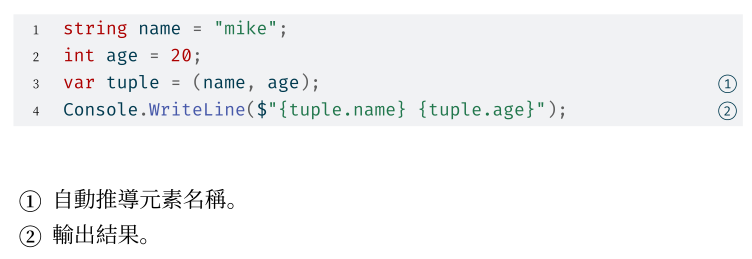
\includegraphics[keepaspectratio]{images/code-annotation-pdf.png}}

\bookmarksetup{startatroot}

\chapter*{參考文獻}\label{ux53c3ux8003ux6587ux737b}
\addcontentsline{toc}{chapter}{參考文獻}

\markboth{參考文獻}{參考文獻}

這裡用來放參考文獻或附錄。

\section*{書籍}\label{ux66f8ux7c4d}
\addcontentsline{toc}{section}{書籍}

\markright{書籍}

\begin{itemize}
\tightlist
\item
  Hadley Wickham, \emph{R for Data Science}, O'Reilly Media, 2017.
\item
  Norman Matloff, \emph{The Art of R Programming}, No Starch Press,
  2011.
\end{itemize}

\section*{網站}\label{ux7db2ux7ad9}
\addcontentsline{toc}{section}{網站}

\markright{網站}

\begin{itemize}
\tightlist
\item
  \href{https://quarto.org}{Quarto 官方文件}
\item
  \href{https://pandoc.org/MANUAL.html}{Pandoc User's Guide}
\end{itemize}


\backmatter


\end{document}
